\documentclass[Main.tex]{subfiles} 


\begin{document}

\subsection{Results}
This experiment was intended to be an anchoring experiment. However, by checking the results we also saw other theories from Kahneman book  put in practice. The results presented in the following sections correspond to 40 participants and the answers were collected from 4/12/2013 to 5/12/2013. The survey is still online and we continue gathering data.

\subsubsection{Anchoring}
The way to introduce the anchors in out survey was a challenge. Our goal was to present it without drawing a lot of attention on it, so a participant would not reject it. We introduced the survey by explaining that its goal is to test the results of a previous prototype session and we provided the average for every feature. We decided to show the current score on the side of each question because people are familiar with ratings since they are used a lot on the internet.

The choice of the anchors was tricky because we wanted them to be believable according to our intuition but we also wanted to preserve a distance between the anchors to  get more noticeable results. We decided to approach this separately for each feature and play with different distances.

Although the features were the target questions of our anchoring experiments, in order to be consistent we used the anchors in the general questions too. In this case, we were more careful to provide more believable anchors in order to establish the trust of the participant to the anchors. In Figures~\ref{fig:general} and~\ref{fig:features} we can see the results of each survey and how the anchoring affects the results.

\begin{figure}
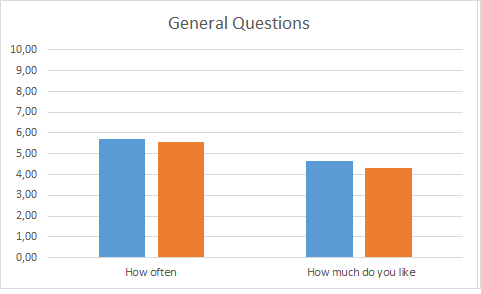
\includegraphics[width=\textwidth]{GeneralQuestions.png}
\caption{The average of the answers to the general questions.}
\label{fig:general}
\end{figure}

\begin{figure}
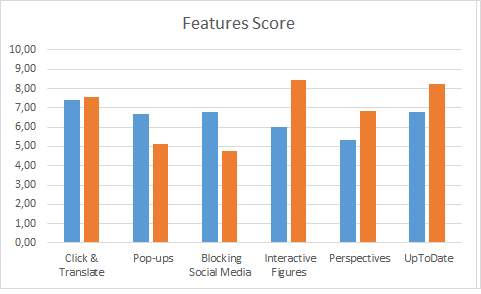
\includegraphics[width=\textwidth]{Featerus.png}
\caption{The average of the answers to the feature questions.}
\label{fig:features}
\end{figure}

\paragraph{Anchoring Index.}%The anchoring effect is explained on page xxx of Kahneman. 
The anchoring effect is measured in percentages by dividing the differences between averages by the difference between the anchors and is called anchoring index. For example, the difference between the anchors 3 and 9 is 6 and the difference between the averages 5 and 7 is 2. Then, the anchoring effect is 2/6, or 30\%. An anchoring effect of 100\% means the subjects adapts the anchor point and an anchoring effect of 0\% means the anchor has no effect on people. 

\begin{figure}
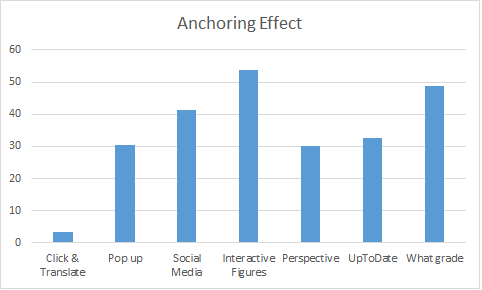
\includegraphics[width=\textwidth]{Anchoringpictures}
\caption{Anchoring index for each feature.}
\label{fig:anchoringIndex}
\end{figure}

In Figure~\ref{fig:anchoringIndex} we see that there was almost no anchoring affect on the question about the dictionary feature (only 3.5\%). This is probably because students already know the feature and like it. We will further discuss that in the following section.

The question about the interactive figures had a very strong anchoring effect, it was 53\%. This is probably one of the examples that people in general do not have a high opinion of so they are easily influenced by the anchor.

Overall we can conclude the anchors did effect the answers to the questions in almost all of the questions. Therefore, no anchors should be put when doing an prototype session. If people do not have a very strong opinion about the prototype they might adjust towards the anchor and the results will not be entirely true.


\subsubsection{Group Dynamics \& Strong Opinions}
Figure~\ref{fig:anchoringIndex} shows that the anchoring effect is not the same in all the questions. We noticed by talking with some participants that they are more drawn to the anchor when they do not have a strong opinion about a feature. This could be explained by group dynamics. The participant prefers to follow the average, the opinion of the group. On the other hand, when  participants are strongly opinionated on a subject, we noticed that they also get affected by the anchor but in the opposite way. Instead of changing their answer towards the anchor they drive it away. When we asked why they did that their answer was that they thought that the rate of this specific feature was really unfair so they wanted to change the average towards their opinion. 

\subsubsection{Availability Heuristic}
The last question of the survey was asking the participants to rate the whole eTextbook. In this question we noticed that the survey that ended with the bad results and was anchored also lower had lower ratings, whereas the other survey  had a higher rating (see Figure~\ref{fig:final}). We believe that this result is a combination of the anchoring and the availability heuristic since the participants could easier recall the last features. 

\begin{figure}
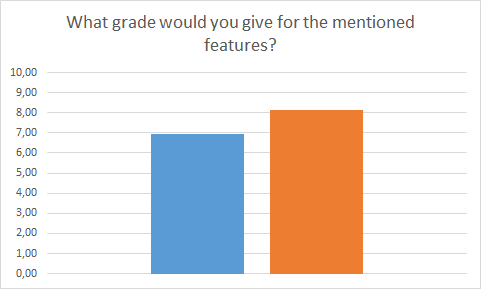
\includegraphics[width=\textwidth]{FinalGrade.png}
\caption{Overall rating of the features.}
\label{fig:final}
\end{figure}

\subsection{Conclusion}
The conclusions of this experiment verified the following guidelines. In order to eliminate the influence from group dynamics the participants should not be able to exchange opinions during the prototype session. Additionally, information that indicates current rating or opinions about the prototype should not be given to participants to avoid anchoring.

%\subsection{Trigger Critical Thinking}
\end{document}